\chapter{方法}
\label{cha:method}
记来自源域的带标注数据集为$\mathbb{D}_s = \{x^s_i, y_i^s\}_{i=1}^{m_s}$,其中$x_i^s\in \mathbb{R}^{w\times h \times 3},y_i^s\in \mathbb{R}^{w\times h\times c}$,$c$是图像中具有不同语义结构的数目,$m_s$表示源域数据集的大小。记来自目标域的无标注数据集$\mathbb{D}_t=\{x_i^t\}_{i=1}^{m_t}$,$m_t$表示目标域数据集的大小。我们旨在利用带标注的源域数据集来对目标域的医学图像进行语义分割。这篇文章将图像的特征进行解耦,从而学习到两个域的解剖学特征和模态特征,文章提出的框架如图\ref{fig:network}所示。对于每个模态的图像,首先利用编码器得到对应域的解剖学特征以及模态特征,然后交换各自的模态特征,将相应的解剖学特征和模态特征输入到解码器得到另一个模态的图像。参考CycleGAN,重复编码解码的操作对原图像进行重构。%\footnote{开源代码:\url{https://github.com/Lawliet-Xie/undergraduate-thesis}}

\section{利用解耦表示来进行图像自适应}
不同模态的医学图像通常具有相似的解剖学结构,即域不变特征,二者的差异往往来自于其不同的模态特征,即域特定的特征。将这些特征进行解耦,进而实现跨模态图像之间的转换。如图所示,编码器$E_d^{anatomy}$和$E_d^{modality}$(下文将解剖学特征anatomy简记为a,模态特征modality简记为m)分别提取图像的解剖学特征以及模态特征,数学形式的表达即$z_d^{c} = E^c_d{x^d}$,其中$c\in \{a,m\}, d\in \{s,t\}$。为了实现解耦表示,常用的方法是通过权重共享将跨模态图像的解剖学特征映射到同一个空间,然而,权重共享很难保证编码出相同的解剖学特征表示。这里引入判别器$D_a$来隐式地对齐跨域的域不变特征,其对抗损失为
\begin{align}
\begin{aligned}L_{\mathrm{adv}}^{\text {a }} &=\mathbb{E}_{x_s}\left[\frac{1}{2} \log D_a\left(z_s^a\right)+\frac{1}{2} \log \left(1-D_a\left(z_s^a\right)\right)\right] \\&+\mathbb{E}_{x_t}\left[\frac{1}{2} \log D_a\left(z_t^a\right)+\frac{1}{2} \log \left(1-D_a\left(z_t^a\right)\right)\right].\end{aligned}
\end{align}
得到解耦表示后,两个域特定的解码器,记为$G_s$,$G_t$,用于生成两个模态的伪图。如图所示,$G_s$可以结合源域图像$x_s$的模态特征和目标域图像$x_t$的解剖学特征来生产伪图$x_s^*=G_s(z_s^{m},z_t^{a})$,同理,我们可以利用$D_t$得到$x_t^*=G_t(z_t^{m},z_s^{a})$。启发于CycleGAN,重复该过程对原图像进行重构,得到$x_s^{\mathrm{rec}}$和$x_t^{\mathrm{rec}}$,即$x_s^{rec} = G_s(E_s^{m}(x_s^*),E_t^{a}(x_t^*)), x_t^{rec} = G_t(E_t^{m}(x_t^*),E_s^{a}(x_s^*))$。这些重构的图像应与原图像一致,故有循环一致性损失(cycle consistency loss):
\begin{align}
\mathcal{L}_{cyc} = \mathbb{E}_{(x_s,x_t)\in P(\mathbb{D}_s,\mathbb{D}_t)}\|x_s^{rec}-x_s\|_1 + \mathbb{E}_{(x_s,x_t)\in P(\mathbb{D}_s,\mathbb{D}_t)}\|x_t^{rec}-x_t\|_1 .
\end{align}
其中$\|\cdot \|_1$代表$\mathrm{L}_1$范数。
\begin{figure}
    \centering
    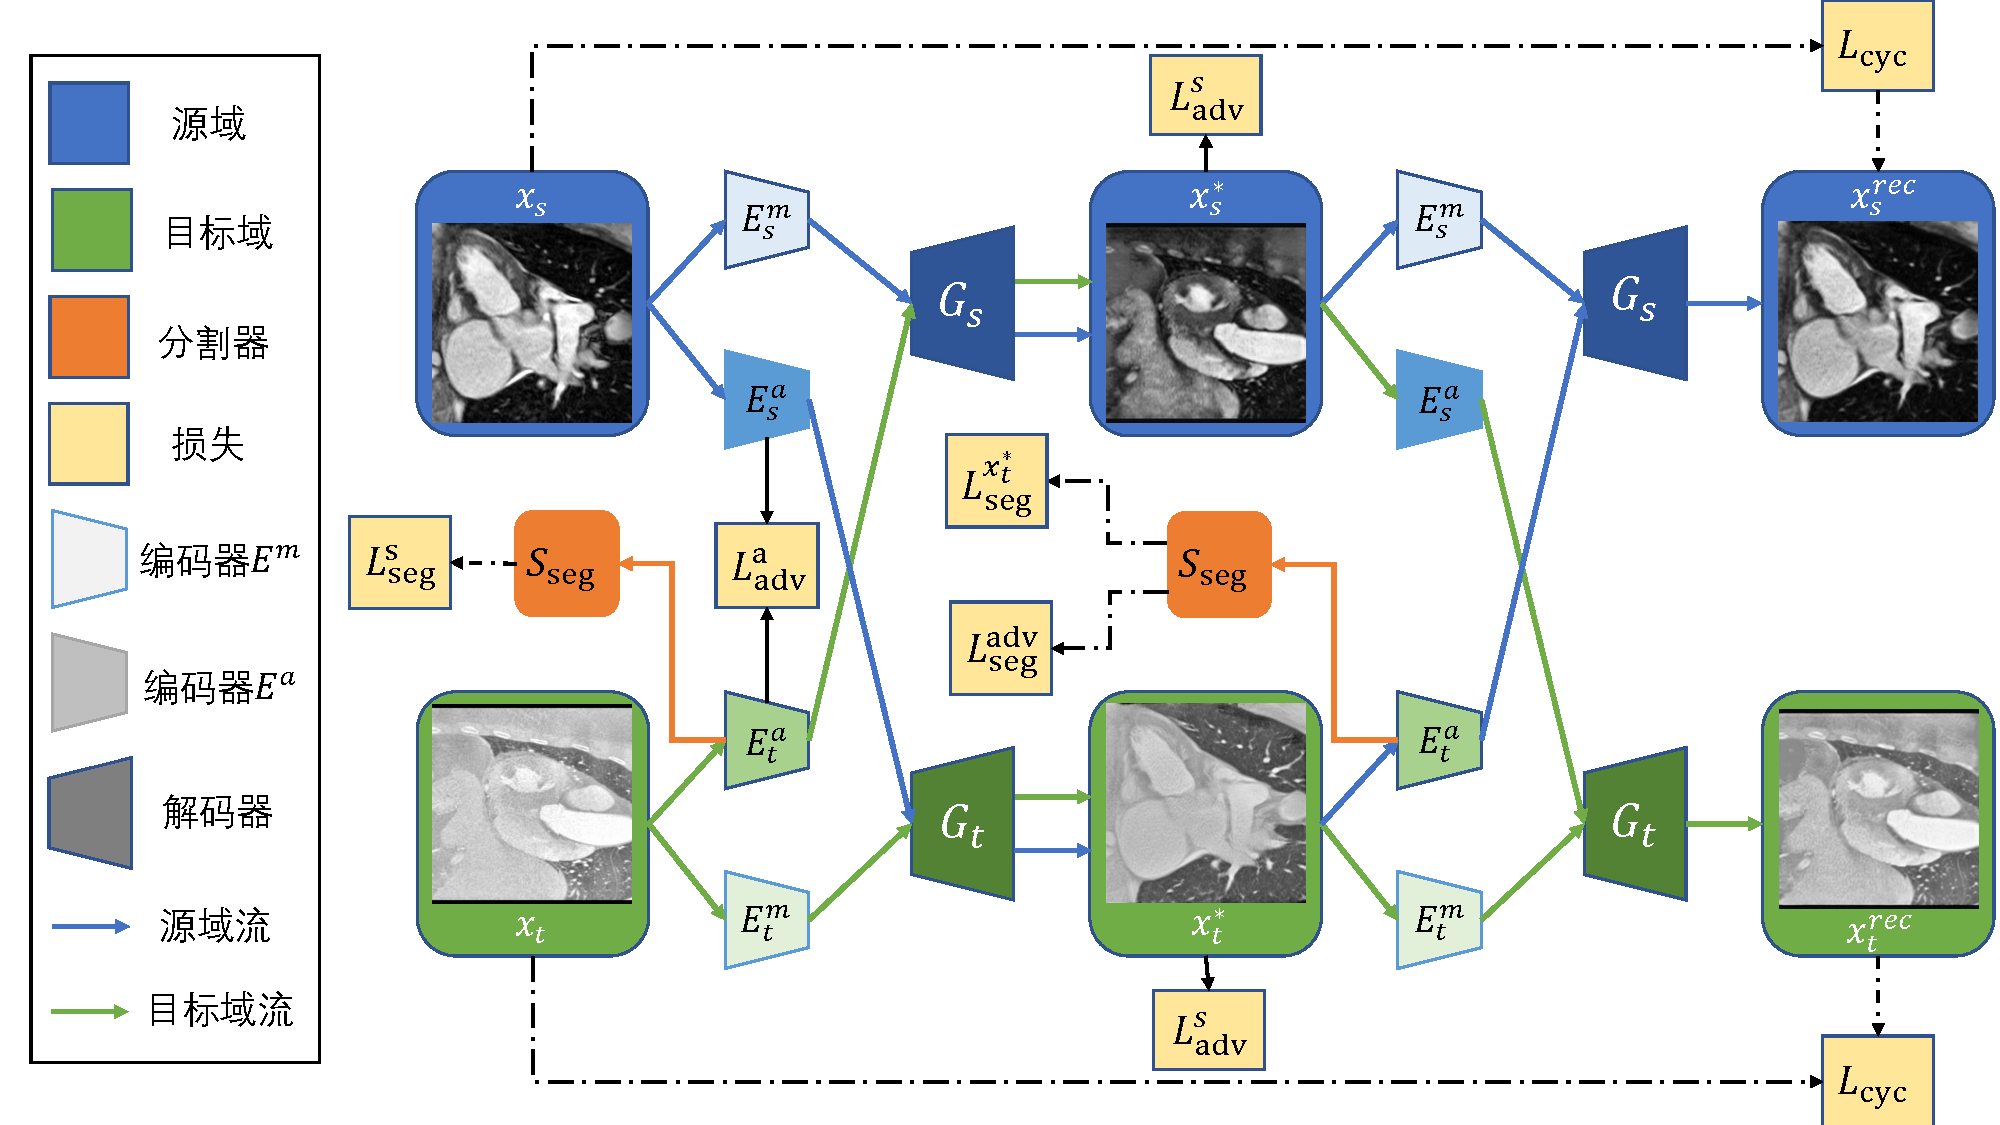
\includegraphics[width=\textwidth]{image/chap03/network structure.pdf}
    \caption{本文整体网络结构}
    \label{fig:network}
\end{figure}
此外,为了使得伪图$x_s^*$和$x_t^*$接近于真实的图像,引入两个判别器$D_s$和$D_t$和以下目标函数用于对抗学习:
\begin{align}
&\min_{(E_s^{a},E_t^{m},G_t)}\max_{D_t} \mathcal{L}_{adv}^t= \mathbb{E}_{x_t\in P(\mathbb{D}_t)}[\log D_t(x_t)] + \mathbb{E}_{(x_s,x_t)\in P(\mathbb{D}_s,\mathbb{D}_t)}[\log (1-D_t(x_t^*))],\\
&\min_{(E_t^{a},E_s^{m},G_s)}\max_{D_s} \mathcal{L}_{adv}^s= \mathbb{E}_{x_s\in P(\mathbb{D}_s)}[\log D_s(x_s)] + \mathbb{E}_{(x_s,x_t)\in P(\mathbb{D}_s,\mathbb{D}_t)}[\log (1-D_s(x_s^*))].
\end{align}
基于生成对抗网络的思想,判别器$D_s$能够分别出$x_s$是真图,而$x_s^*$是伪图,同时以上的由编码器解码器组成的生成器结构能够生成出足够真实的样本来干扰判别器,$D_t$同理。

\section{网络结构}
\subsection{编码解剖学特征}
解耦解剖学特征的编码器由卷积神经网络组成,将2D的医学图像映射到其空间表示,即$E^a:x\rightarrow z^a$,其中$z^a\in \mathbb{R}^{w\times h\times k}$,k表示所需要的解剖学特征数。编码器整体采用类似U-Net\cite{ronneberger2015u}的网络结构,如图\ref{fig:enc_anatomy}所示,包含了下采样,上采样以及跳跃连接,能够有效地融合重要的局部和非局部信息,提取出丰富的语义信息,得到特征中的每个通道表示心脏中一些具有解剖学意义的子结构。
\begin{figure}
    \centering
    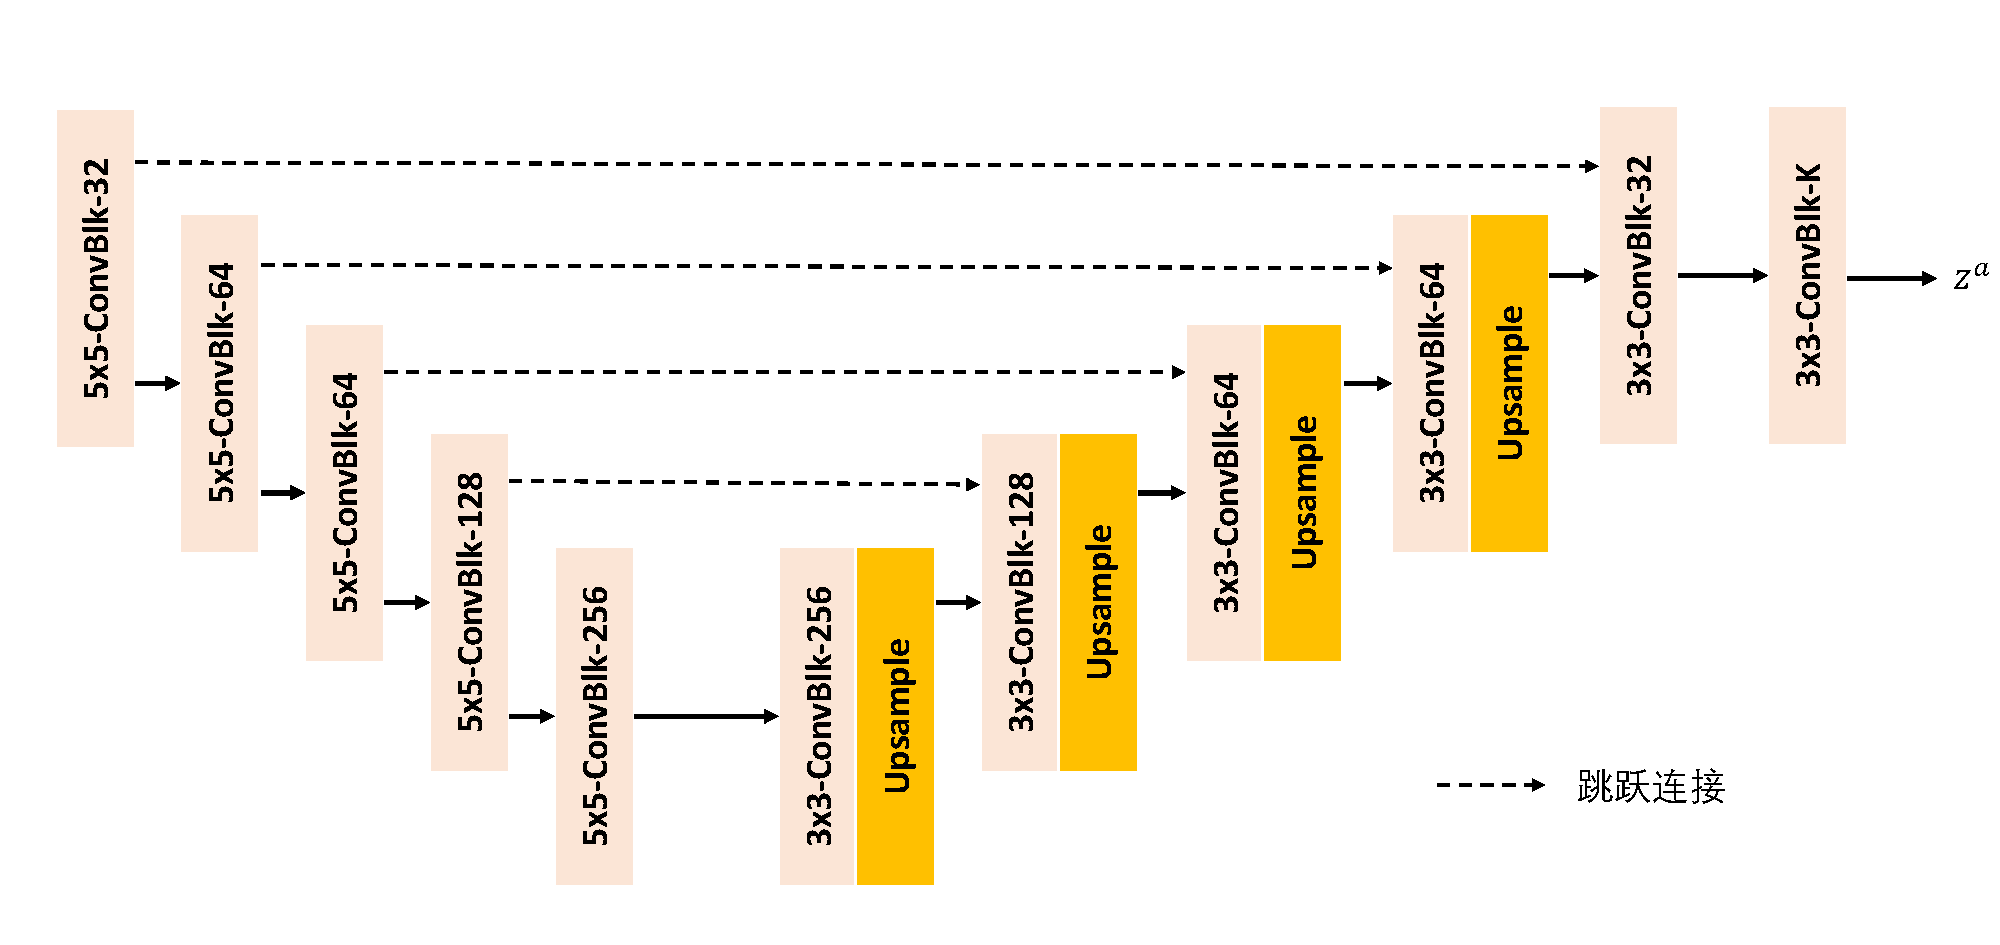
\includegraphics[width=\textwidth]{image/chap03/encoder_anatomy.pdf}
    \caption{解剖学特征编码器}
    \label{fig:enc_anatomy}
\end{figure}
\subsection{编码模态特征}
编码器$E^m$为了学习到医学图像模态特征$z^m$的后验分布$q(z^m|x)$,采用变分自编码器\cite{kingma2013auto}(Variational Autoencoder, VAE)。简单地说,VAE学习一个低维的潜空间,该特征空间中的潜表示能够匹配一个先验分布$p(z)=\mathcal{N}(\bold{0},I)$,从风格迁移和解耦表示的角度来说,从该空间中进行模态的采样,能够生成各种模态的图像,整体结构如图\ref{fig:enc_modality}所示。
\begin{figure}
    \centering
    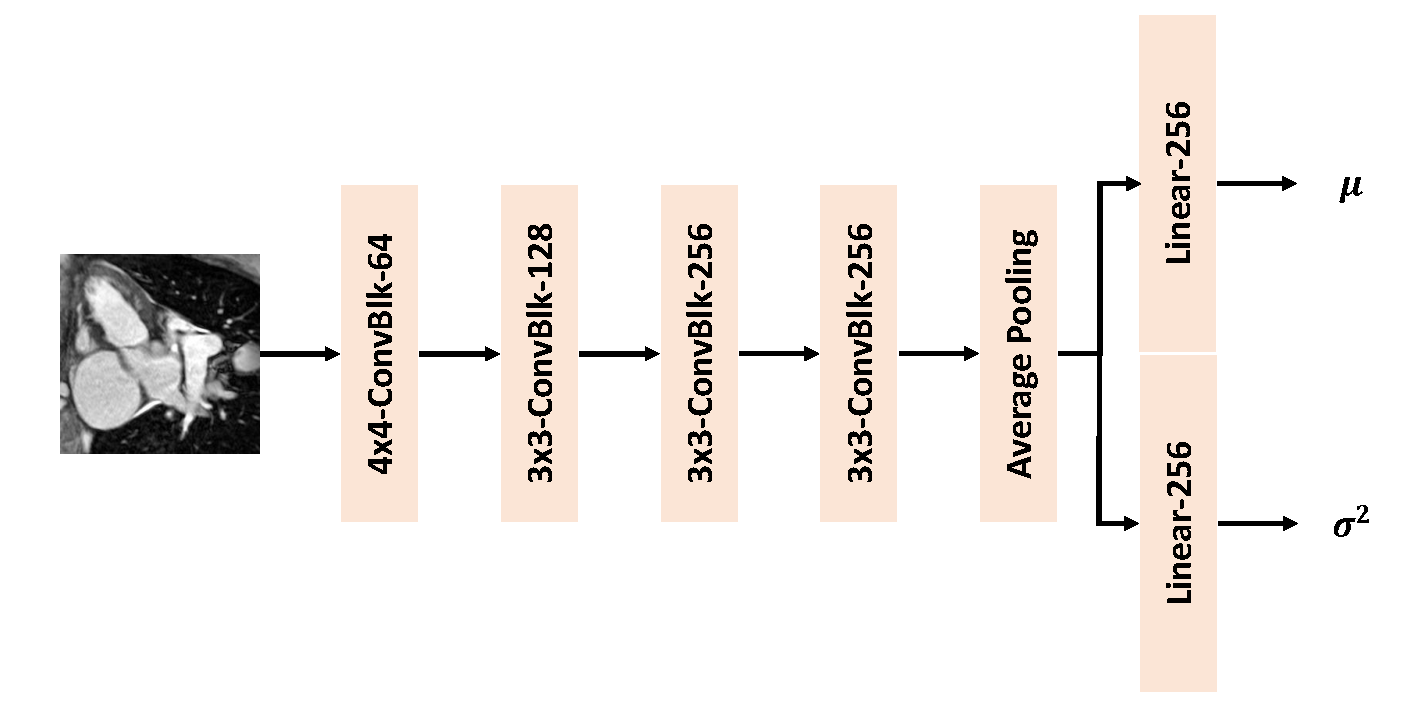
\includegraphics[width=\textwidth]{image/chap03/encoder_modality.pdf}
    \caption{模态特征编码器}
    \label{fig:enc_modality}
\end{figure}

\subsection{解码器}
解码器$G$以模态特征和解剖学特征作为输入,用于进行图像的生成与重构。SPADE\cite{park2019semantic}(Spatially Adaptive Denormalization)是一种能有效利用语义信息以及风格信息进行图像生成的一种结构。与普通的卷积神经网络对比,其通过空间自适应归一化来更好地保留语义信息,具体公式如下:
\begin{align}
    \begin{split}
    \hat{x}_{c,i,j}(z^a) &=\gamma_{c,i,j}(z^a) * \frac{z^m_{c,i,j}-\mu_{c}}{\sigma_{c}}+\beta_{c,i,j}(z^a) \\
    \mu_{c} &=\frac{1}{H W} \sum_{i, j} z^m_{c,i,j},\quad \sigma_{c}^{2}=\frac{1}{H W} \sum_{i, j}\left(z^m_{c,i,j}-\mu_{c}\right)^{2}
    \end{split}
\end{align}
在该模块中,解剖学特征$z^a$被映射到一个嵌入空间来产生仿射变换的参数$\gamma$和$\beta$,不同于AdaIN等其他条件归一化方法,SPADE产生的$\gamma$和$\beta$包含了空间和相应的语义信息,接着利用$\gamma$和$\beta$对已经实例归一化的模态特征$z^m$来实现多模态的图像生成\cite{park2019semantic},如图\ref{fig:spade}所示。解码器(图\ref{fig:decoder})由多个SPADE块组成,能够充分融合解剖学特征和模态特征来进行伪图的生成以及原图的重建。
\begin{figure}
    \centering
    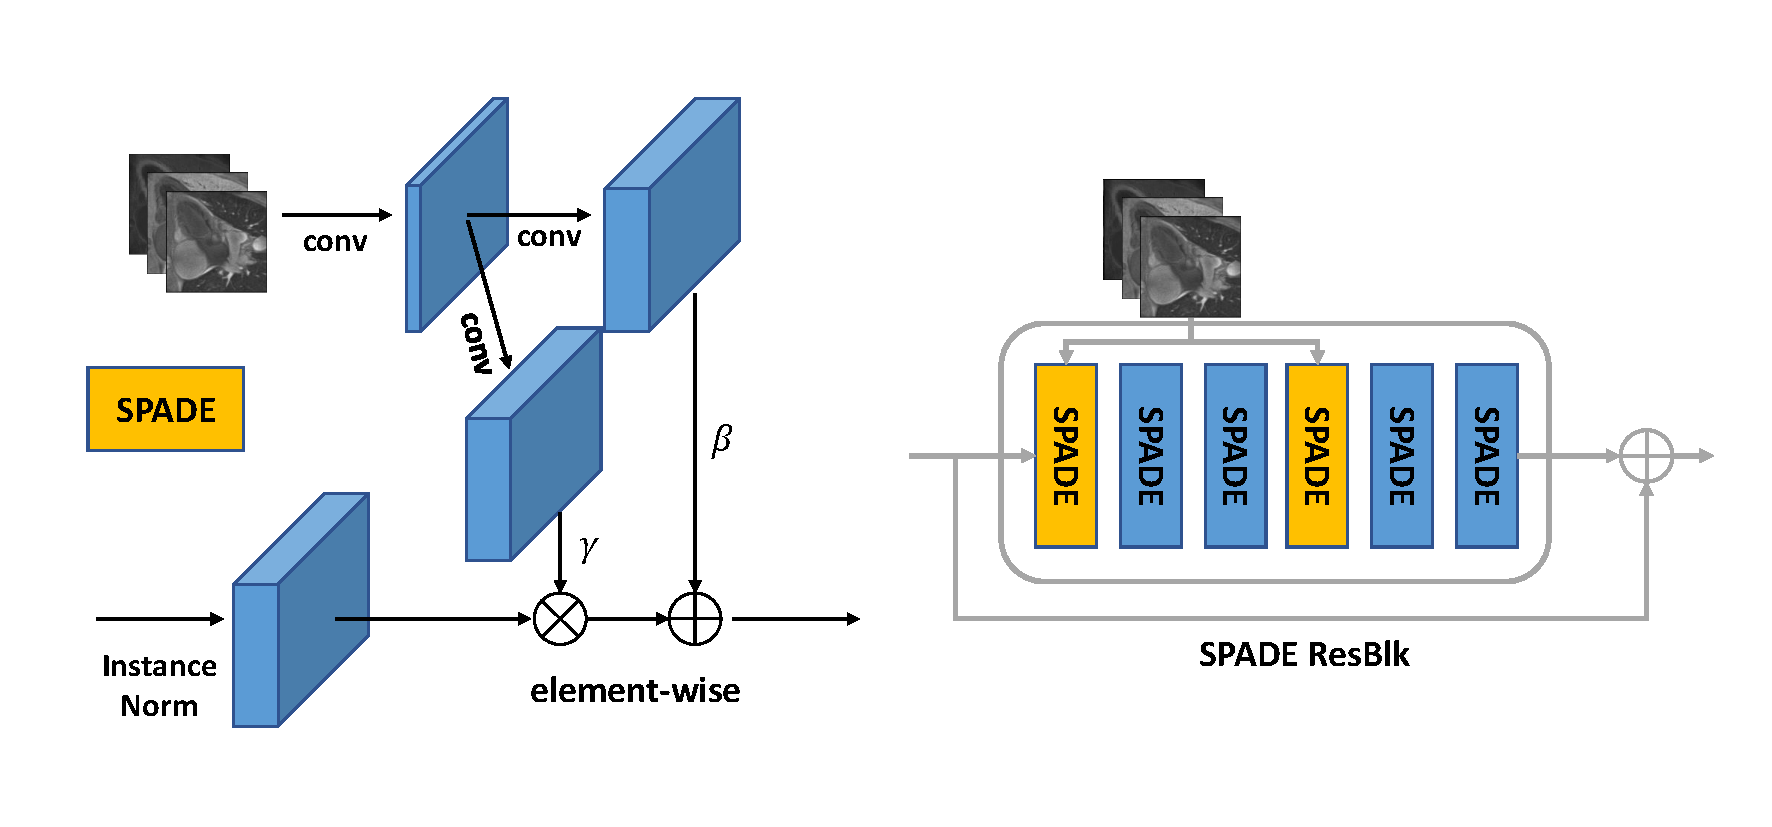
\includegraphics[width=\textwidth]{image/chap03/SPADE.pdf}
    \caption{SPADE网络结构}
    \label{fig:spade}
\end{figure}
\begin{figure}
    \centering
    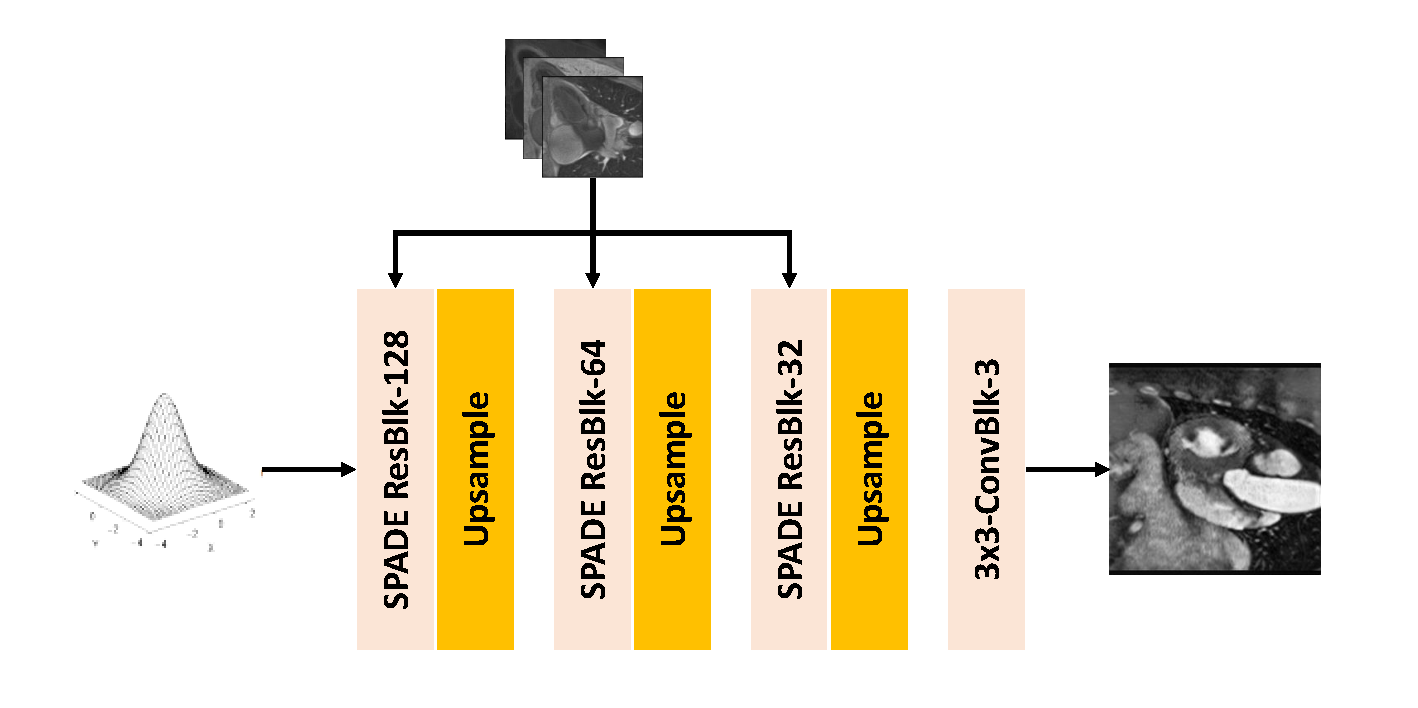
\includegraphics[width=\textwidth]{image/chap03/decoder.pdf}
    \caption{由SPADE ResBlock组成的解码器结构}
    \label{fig:decoder}
\end{figure}

\subsection{分割器}
解剖学特征已经包含了医学图像中丰富的语义信息,在此基础上增加一层卷积神经网络$S_{\mathrm{seg}}$来完成语义分割。由于源域图像带标注$y_s$,生成的伪图$x_t^*$与$x_s$共享相似的解剖学特征$z_s^a$,故$S_{\mathrm{seg}}$对二者的分割预测$\hat{y}_{t^*}$和$\hat{y}_s$能够与$y_s$进行监督学习,有如下损失:
\begin{align}
    \mathcal{L}_{\text {seg }}^{x_s}=\mathcal{H}\left(y_{s}, \hat{y}_{s}\right)+\alpha \cdot \operatorname{Dice}\left(y_{s}, \hat{y}_{s}\right),\\
    \mathcal{L}_{\text {seg }}^{x_t^*}=\mathcal{H}\left(y_{s}, \hat{y}_{t^*}\right)+\alpha \cdot \operatorname{Dice}\left(y_{s}, \hat{y}_{t^*}\right).
\end{align}
其中$\mathcal{H}$为交叉熵损失,$\operatorname{Dice}$损失用于衡量语义分割效果,具体计算公式见附录,$\alpha$为超参数。总的分割损失可表示为$\mathcal{L}_{\mathrm{seg}} = \mathcal{L}_{\text {seg }}^{x_s} + \mathcal{L}_{\text {seg }}^{x_t^*}.$
此外,引入判别器$D_{\mathrm{seg}}$,进一步从语义空间上缩小源域和目标域图像的分布差异,
\begin{align}
    \begin{aligned}\min _{\left(E_{t}^a, S_{\text {seg }}\right)} \max _{D_{\mathrm{seg}}} \mathcal{L}_{a d v}^{\operatorname{seg}}&=\mathbb{E}_{x_{t}^{*}}\left[\log D^{\mathrm{seg }}\left(S_{\text {seg }}\left(E_{t}^a\left(x_{t}^{*}\right)\right)\right)\right] \\&+\mathbb{E}_{x_{t} }\left[\log \left(1-D_{\mathrm{seg}}\left(S_{\text {seg }}\left(E_{t}^a\left(x_{t}\right)\right)\right)\right)\right] .\end{aligned}
\end{align}

\section{正则约束}
\begin{itemize}
    \item 正交约束\\对得到的解剖学特征进行正交性约束,使得每个通道能学习到不同病理意义的子结构,减少特征的冗余性,更好地解耦解剖学特征和模态特征。
    \begin{align}
        \mathcal{L}_{\text {ortho}}=\mathbb{E}_{x_s}\left[\left\|E^a_s(x_s) E^a_s(x_s)^T-I\right\|_{F}\right] + \mathbb{E}_{x_t}\left[\left\|E^a_t(x_t) E^a_t(x_t)^T-I\right\|_{F}\right].
    \end{align}
    其中$I$是单位矩阵,$\|\cdot \|_F$代表Frobenius范数。
    \item KL散度约束\\该损失函数目的是使模态表示$q(z^m|x)=\mathcal{N}(\mu(x), \sigma(x)^2)$与先验高斯分布$p(z)=\mathcal{N}(\bold{0},I)$一致,从图像生成的角度,我们从该先验高斯分布中随机采样,能得到不同模态的图像。
    \begin{align}
        \begin{aligned}\mathcal{L}_{\mathrm{KL}}&=\mathcal{D}_{\mathrm{KL}}(q(z^m|x)\|p(z))\\&=-\int{q(z^m|x)\log\frac{q(z^m|x)}{p(z)}dz}\\&=\frac{1}{2}\sum_{j=1}^d(\sigma_j+u_j^2-\log \sigma_j-1).\end{aligned}
    \end{align}
    \item 重构约束\\除了交叉循环重构损失,以$E_s^a$和$E_s^m$为输入,进入解码器$G_s$理应能重构出原来的图像$x_s$,对于目标域图像$x_t$同理,即如下重构损失:
    \begin{align}
        \mathcal{L}_{\mathrm{id}} = \mathbb{E}_{x_s}[\|G_s(E_s^a(x_s),E_s^m(x_s))-x_s\|_1] + \mathbb{E}_{x_t}[\|G_t(E_t^a(x_t),E_s^m(x_t))-x_t\|_1].
    \end{align}
\end{itemize}
结合以上提到的损失函数,总的目标函数为
\begin{align}
    \begin{aligned}
    \mathcal{L} &= \lambda_1\mathcal{L}_{adv}^a +\lambda_2\mathcal{L}_{cyc} +\lambda_3\mathcal{L}_{adv}^s +\lambda_4\mathcal{L}_{adv}^t \\
    &+\lambda_5\mathcal{L}_{\mathrm{seg}} +\lambda_6\mathcal{L}_{adv}^{\mathrm{seg}} +\lambda_7\mathcal{L}_{\mathrm{ortho}} +\lambda_8\mathcal{L}_{\mathcal{\mathrm{KL}}} + \lambda_9\mathcal{L}_{id}.
    \end{aligned}
    \label{eq:loss}
\end{align}
其中,$\lambda_1\sim \lambda_9$为超参数,用于平衡各个模块的重要性。第一项损失旨在使得源域和目标域图像能够提取到域不变特征,第二项和最后一项损失旨在重构回原来的图像,第三第四项损失旨在生成足够真实的伪图从而能够干扰判别器,第五项为利用监督学习进行语义分割产生的损失,其余项的提出是为了促进不同模态图像之间域自适应,缓解域位移问题。

\section{实现细节}
这一小节我们补充训练过程中各种参数的设定以及相应模块的网络结构设置。

在训练过程当中,对分割器模块使用初始学习率为$1\times 10^{-3}$的Adam优化器,学习率以每两个epoch以0.9的倍率进行衰减,对于其他模块则以恒定的$2\times 10^{-4}$的学习率进行随机梯度下降更新参数,总训练epoch数为50,数据批量大小为8。

每个模块基于卷积神经网络块(ConvBlock),由$3\times 3$卷积核的CNN,实例归一化以及参数为$0.2$的leaky RELU组成。为了生成对抗网络训练的稳定性,参照CycleGAN的设定,我们使用了基于均方误差的对抗损失。此外,对引入的四个判别器,采用PatchGAN\cite{isola2017image}的设置对$70\times 70$的补丁进行判别。

关于超参数的设定,$\alpha=1, \lambda_1=2, \lambda_2=10, \lambda_3=2, \lambda_4=2, \lambda_5=0.5, \lambda_6=2, \lambda_7=1, \lambda_8=0.01, \lambda_9=2.5$,解剖学特征数$K=8$。在MMWHS数据集上训练的误差如图\ref{fig:loss}所示,图\ref{fig:gen_loss}展示了生成器的训练损失,即式\ref{eq:loss}中总损失减去判别器损失,图\ref{fig:dis_loss}则展示了判别器在训练过程中的损失。
可以看到,生成器损失随着迭代次数不断下降,意味着框架能生成足够真实的伪图以及解剖学特征编码器能编码出域不变的特征,而判别器损失则先降后增,说明训练阶段初期判别器能够分辨出真图和伪图,而到了后期,由于生成器能够生成足够真实的图像来干扰判别器,使得判别器的损失回升。

\begin{figure}
    \centering
    \begin{subfigure}{0.45\textwidth}
        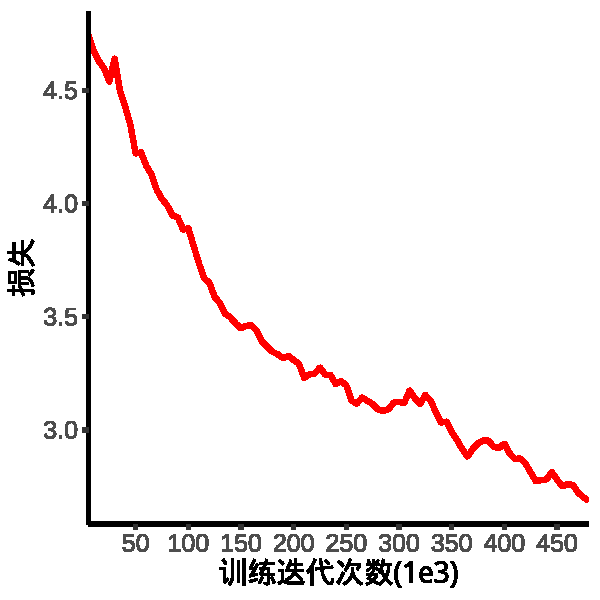
\includegraphics[width=\textwidth,height=\textwidth]{image/chap03/gen_loss.pdf}
        \caption{生成器训练损失}
        \label{fig:gen_loss}
    \end{subfigure}
    \hfill
    \begin{subfigure}{0.45\textwidth}
        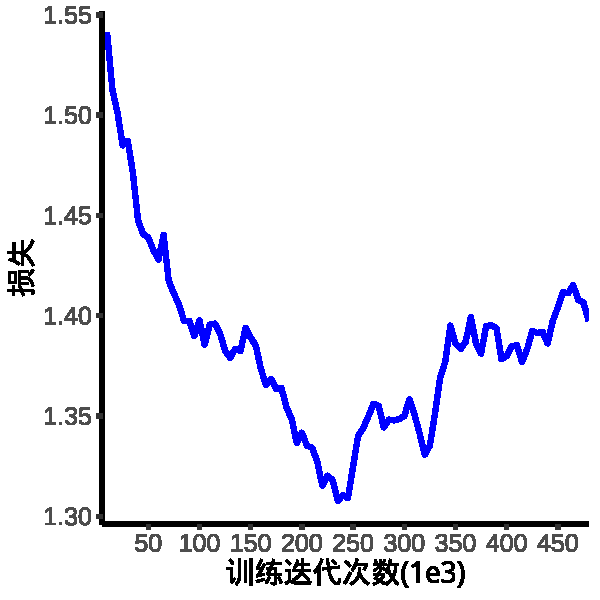
\includegraphics[width=\textwidth,height=\textwidth]{image/chap03/dis_loss.pdf}
        \caption{判别器训练损失}
        \label{fig:dis_loss}
    \end{subfigure}
    \caption{在MMWHS数据集上进行训练的损失}
    \label{fig:loss}
    \end{figure}
